\documentclass[12pt,a4paper]{IEEEtran}
\usepackage{cite}
\usepackage{graphicx}
\usepackage[cmex10]{amsmath}
 \interdisplaylinepenalty=2500
\usepackage[caption=false,font=footnotesize]{subfig}
\usepackage{fixltx2e}
\usepackage{hyperref}
\usepackage{listings}
\usepackage{tabularx}

% Make captions look better.
\usepackage{caption}
\captionsetup{margin=30pt,font=small,labelfont=bf}

\title{What's New in SIMD Design}

\author{
  \begin{tabular}{ccc}
    Daniel Bentall & Simon Richards & Henry Jenkins \\
    \href{mailto:djb216@uclive.ac.nz}{\texttt{djb216@uclive.ac.nz}} &
    \href{mailto:scr52@uclive.ac.nz}{\texttt{scr52@uclive.ac.nz}} &
    \href{mailto:hvj10@uclive.ac.nz}{\texttt{hvj10@uclive.ac.nz}} \\

     & & \\

    Benjamin Washington-Yule & Zachary Taylor & Wim Looman \\
    \href{mailto:byu17@uclive.ac.nz}{\texttt{byu17@uclive.ac.nz}} &
    \href{mailto:zjt14@uclive.ac.nz}{\texttt{zjt14@uclive.ac.nz}} &
    \href{mailto:wgl18@uclive.ac.nz}{\texttt{wgl18@uclive.ac.nz}} \\
  \end{tabular}

  \vspace{14pt}

  \IEEEauthorblockN{
    \emph{Supervisor}: Dr. Steve Weddell\\
    \href{mailto:steve.weddell@canterbury.ac.nz}{\texttt{steve.weddell@canterbury.ac.nz}}
  }

  \vspace{14pt}

  \IEEEauthorblockA{
    Department of Electrical and Computer Engineering\\
    University of Canterbury\\
    Christchurch, New Zealand
  }
}


\begin{document}

  \maketitle

  \begin{abstract}
This report explores the implementation and testing of a Single Instruction
Multiple Data (SIMD) Accumulator based CPU on a Xilinx FPGA development board.
\end{abstract}

  \section{Introduction}

\IEEEPARstart{W}{hat} is SIMD would probably be a better place to start.  This
report will detail exactly what SIMD is and why it is still useful in designing
new CPU cores.  This will be done in the context of the
TREVA\footnote{\url{https://github.com/team-ramrod/treva}} project --
\emph{Team-Ramrod's ENEL429 VHDL Assignment}.

One of the possible applications that was being explored was the implementation
of a Fast Fourier Transform \cite{Jamieson198648}.

%TODO: Introduce what's new in SIMD then what's in our report

\subsection{Spartan 3E-1600E}
% Talk about the board/FPGA we used


  \section{Background}
\subsection{SIMD}

\subsection{Leros}
In order to avoid carrying out redundant work, a decision was made to utilise an
existing solution as a base development. The advantages were twofold; not only
did it allowed for much faster development, but had already been tested by many
people. Opencores\footnote{
http://www.opencores.com
}
is a large open-source hardware community, well-known for its collection of hardware solutions for
FPGAs and ASICs, in both VHDL and Verilog. Our requirements called for a VHDL
microcontroller, of which there were many to choose from. Other critera included
simplicity of code, small code size, and a RISC architecture. One project stood out
after applying these critera, named the \emph{Leros} microcontroller after the
Greek Island Leros \cite{cite:TODO}.  The Leros MCU is a 16-bit
processor optimized for FPGAs \cite{cite:TODO}, and was selected for use in this
project.

 It is a stable
project and can even be programmed in a restricted subset of Java. It is licenced
under the permissive BSD licence and has been tested under the Xilinx toolchain.
Leros' architecture is a pipelined 16-bit accumulator processor\ref{cite:TODOpdf},
with instructions exectuted in a single cycle.

The accumulator architeuectur made Leros an attractive option for this project.

\begin{figure*}[h]
\center
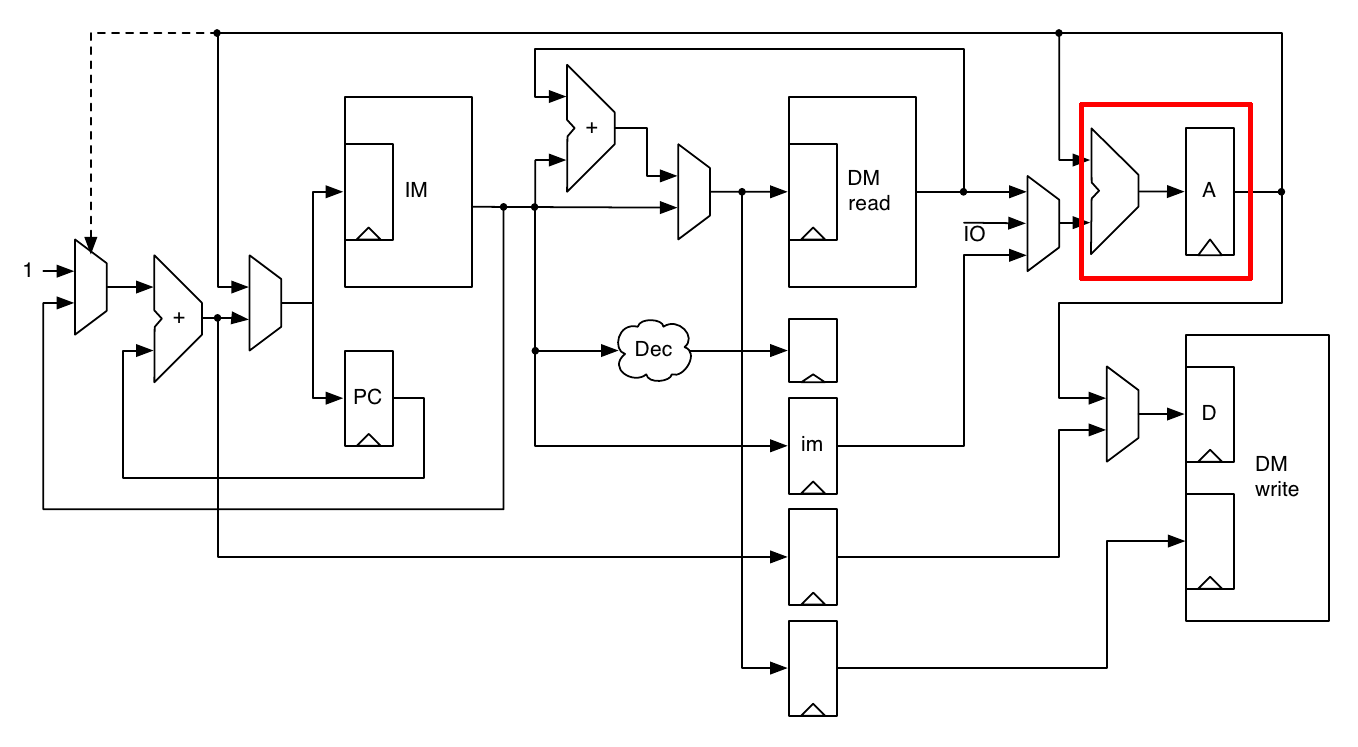
\includegraphics[width=0.9\textwidth]{images/leros-system}
\caption{Leros pipeline. The section of the design to be multiplied has been
highlighted in red. Original image from \cite{cite:TODO-pdf}.
}
\label{fig:leros-system}
\end{figure*}

  \section{Design \& Implementation}
\subsection{Instruction Set Extension}

The Leros microcontroller has a restricted instruction set, lacking multiply or
divide instructions, and shift and rotate operations. A multiplication
instruction was originally required for the project's selected application (a
fast Fourier transform), and therefore required a change to Leros' code. Such a
change was complicated by the structure of Leros' instruction register, which
did not have room for the additional logic to accommodate new operations. Since
the Leros code supports only two arithmetic instructions, a single bit in the
opcode was used to determine whether the instruction was an ADD or a SUB
instruction.

The first 5 bits of the instruction in the Leros CPU corresponded to that shown
in Table \ref{tab:original-instruction}.

\begin{table}
\centering
\caption{The original Leros instruction categories}
\label{tab:original-instruction}
\begin{tabular}{|l|l|}
\hline
\textbf{Bits} & Meaning \\
\hline
\texttt{00000} & NOP \\
\texttt{00001} & Arithmetic Operation (ADD/SUB) \\
\texttt{00010} & Right Shift \\
\texttt{00011} & reserved \\
\texttt{00100} & ALU / Logic Operation \\
\texttt{00101} & Load \\
\texttt{00110} & Store \\
\texttt{00111} & IO \\
\hline
\end{tabular}
\end{table}

Whether the arithmetic instruction was an ADD or SUB was further determined by
the second bit of the instruction. It was decided that this was inefficient and
limiting. However, it was desirable than any changes to the opcode preserved the
majority of the existing form. The instruction format was changed such that the
first 5 bits of the instruction simply set a flag, and the actual operation was
encoded in bits 1 and 2 of the instruction. This is in contrast to the original
Leros code which encodes the arithmetic instruction in one bit, but was limited
to two such instructions. The flag set was defined as a new type and takes one
of three values: \texttt{arith\_flag} for arithmetic operations,
\texttt{logic\_flag} for logic operations, and  \texttt{io\_flag} for IO. This
also left space for an additional four operations should they ever be required.
The additional bit needed to represent the new instructions was obtained by
using one of the bits previously used to represent a logic operation, which
themselves were now represented using the flags mentioned above.

Arranging things thus allowed many more instructions to be included. For each
class of instruction, four operations were possible, giving a total of $4 \times
4 = 16$ operations. This also left space for an additional four operations
should they ever be required. Additionally, it  had the added benefit of
allowing left and right shift and rotate instructions to be added. The Leros
design only supports right-shift; the reason for the original omissions of the other
operations is unknown.



\subsection{Vector ALU}
To perform the vector operations in a single clock cycle extra ALUs had to be added. These ALUs were placed in parallel with the original and each output into its own accumulator. Originally it had been intended that the accumulators would each output onto one $16n$ wide bus where $n$ was the number of ALUs present in the system. This design ran into issues however due to the physical limitations of the memory units on the FPGA. These ram blocks could only support 32 bits being written and read per clock cycle \cite{spartan_ram}. This limited the CPU to either two ALUs or multiple clock cycles per vector operation to access the memory. Both of these options would have resulted in a significant reduction to the maximum speed up obtainable by the CPU over the original design and so another solution was looked for.

This solution came in the form of using dedicated ram for each ALU. This lack of shared ram however introduced a new problem, there was no longer any way for the ALUs to read what was written to the others memory. This problem was solved via the modification of the load store instructions. Initially these instructions communicated with a single I/O port to send and receive from. These instructions contained an unused 8 bit operand that was taken advantage of. This operand was broken up into one 4 bit address operand and one 4 bit memory operand. For the load operation if the operand was one of the memory addresses the value of the addressed data memory would be loaded into the accumulator of all the ALUs through the use of a new data select unit. If a store instruction was used then the output of the addressed ALUs accumulator register would be stored to its memory. This effectively allowed for data to be moved between the data memories. A block diagram of the modifications to the data path mentioned can be seen in Figure~\ref{new_path}.

This new data select unit replaced the data select mux that was placed in front of the ALU. It was required as with the addition of two four bit operands to the load and store instructions and the addition of vector operations the logic controlling this select complicated significantly. These complications meant that a large amount of extra control lines were needed that would only be used by this small section. To mitigate the complication to the logic the decision was made to break the selection of which data to pass into each ALU into its own unit.

\begin{figure*}[ht]
	\begin{center}
		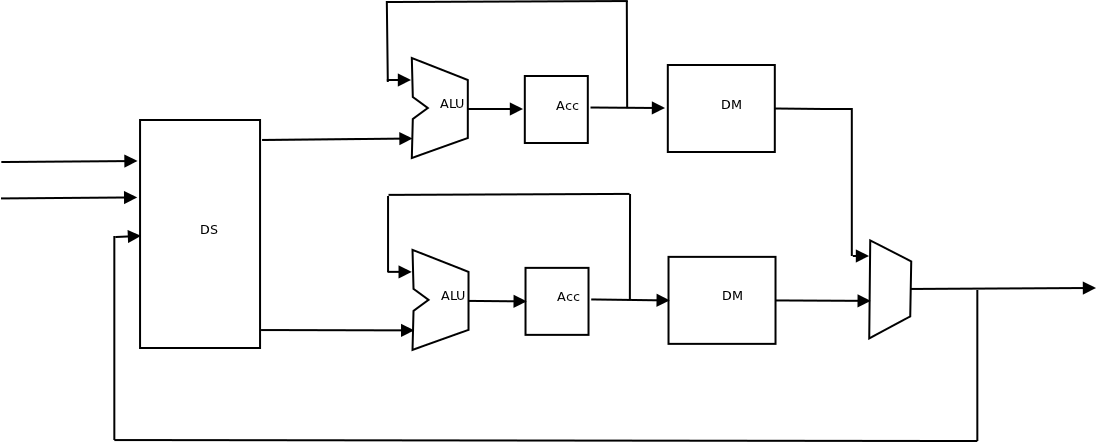
\includegraphics[width=0.8\textwidth]{images/new_path}
	\end{center}
	\caption{A block diagram of the modified area of the leros data path. ACC is the accumulator, DM is the data memory, DS is the data select.}
	\label{new_path}
\end{figure*}

The use of a 4 bit memory address operand limited the maximum number of additional ALUs to 32. A limit was also imposed by the board used as it only contained 36 blocks of ram meaning that even if a larger operand had been used little extra performance would be gained \cite{spartan_ram}. This meant that the board's memory was again acting as the bottleneck for the design as, with the exception of memory, the FPGA contained space to synthesise several hundred ALUs as was the original intent. The only option available at this point  to improve the memory was to use flip-flops instead of the ram. This was highly undesirable for two reasons. Firstly the number of flip-flops that were possible was only around 10,000 \cite{spartan_user}, while this may be more than enough for most applications, when being used as memory this was insufficient for the image processing operations around which the CPU was designed. Secondly, the use of flip-flops rather than the on-board memory meant that the maximum clock speed of the CPU was reduced by around 50\%. Because of these issues the implementation with a limit of 32 ALUs was kept.

The movement of data between memory blocks meant that while the CPU could perform the arithmetic and logical operations in parallel its memory operations could only occur in serial and due to the need to move data between memory blocks a significantly higher number of these load and store operations would be required for the program to perform. How much this affected the speed up of the additional ALUs would be largely program dependent. 

The implementation of several other instructions required alteration to work with the new multiple ALUs. The add and load immediate operations were altered to allow the immediate to be placed on the bus to all the ALUs so that they all performed the operation. All the branching and jumping operations operated only on the first ALU with this ALU being the only one  queried for branch conditionals This was done as with a single control unit the ALUs all had to perform the same instructions and so could not branch to different sections of code.


\subsection{Assembler for VHDL}

  Leros provided us with an assembler, this was based on an ANother Tool for
  Language Recognition (ANTLR) generated Java parser and lexer.  Because of the
  quite major changes that would be required to add in support for vector
  operations, along with no one in the group having experience with ANTLR, it
  was decided that re-writing an assembler in a known language would be useful.

  The re-write was performed using Ruby, a two-pass assembler was created that
  matched the output of the Leros assembler, with one slight difference.  The
  Leros assembler output a VHDL file to synthesis as a ROM, the new assembler
  output a binary file.  To keep the integrated ROM a VHDLiser was also written
  that input the binary and output a VHDL ROM.

  To perform the vector operations in a single clock cycle extra ALUs had to be added. These ALUs were placed in parallel with the original and each output into its own accumulator. Originally it had been intended that the accumulators would each output onto one $16n$ wide bus where $n$ was the number of ALUs present in the system. This design ran into issues however due to the physical limitations of the memory units on the FPGA. These ram blocks could only support 32 bits being written and read per clock cycle \cite{spartan_ram}. This limited the CPU to either two ALUs or multiple clock cycles per vector operation to access the memory. Both of these options would have resulted in a significant reduction to the maximum speed up obtainable by the CPU over the original design and so another solution was looked for.

This solution came in the form of using dedicated ram for each ALU. This lack of shared ram however introduced a new problem, there was no longer any way for the ALUs to read what was written to the others memory. This problem was solved via the modification of the load store instructions. Initially these instructions communicated with a single I/O port to send and receive from. These instructions contained an unused 8 bit operand that was taken advantage of. This operand was broken up into one 4 bit address operand and one 4 bit memory operand. For the load operation if the operand was one of the memory addresses the value of the addressed data memory would be loaded into the accumulator of all the ALUs through the use of a new data select unit. If a store instruction was used then the output of the addressed ALUs accumulator register would be stored to its memory. This effectively allowed for data to be moved between the data memories. A block diagram of the modifications to the data path mentioned can be seen in Figure~\ref{new_path}.

This new data select unit replaced the data select mux that was placed in front of the ALU. It was required as with the addition of two four bit operands to the load and store instructions and the addition of vector operations the logic controlling this select complicated significantly. These complications meant that a large amount of extra control lines were needed that would only be used by this small section. To mitigate the complication to the logic the decision was made to break the selection of which data to pass into each ALU into its own unit.

\begin{figure*}[ht]
	\begin{center}
		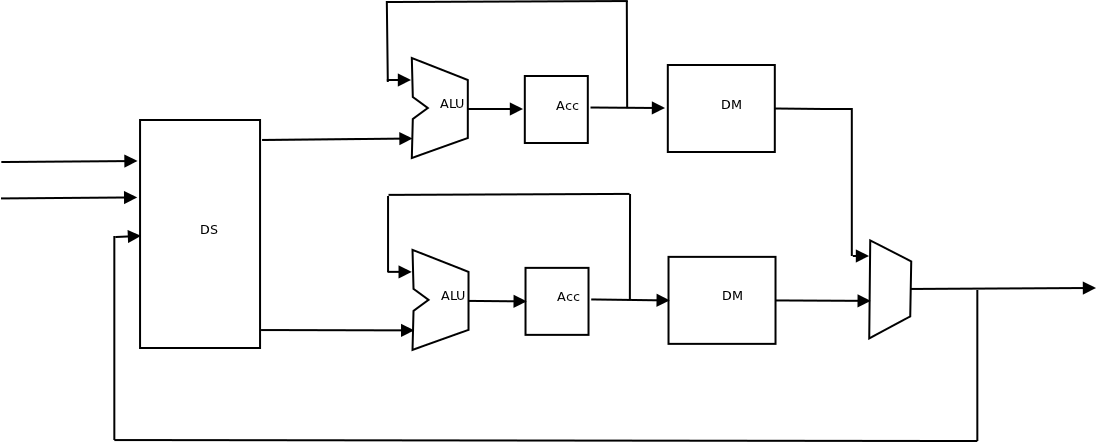
\includegraphics[width=0.8\textwidth]{images/new_path}
	\end{center}
	\caption{A block diagram of the modified area of the leros data path. ACC is the accumulator, DM is the data memory, DS is the data select.}
	\label{new_path}
\end{figure*}

The use of a 4 bit memory address operand limited the maximum number of additional ALUs to 32. A limit was also imposed by the board used as it only contained 36 blocks of ram meaning that even if a larger operand had been used little extra performance would be gained \cite{spartan_ram}. This meant that the board's memory was again acting as the bottleneck for the design as, with the exception of memory, the FPGA contained space to synthesise several hundred ALUs as was the original intent. The only option available at this point  to improve the memory was to use flip-flops instead of the ram. This was highly undesirable for two reasons. Firstly the number of flip-flops that were possible was only around 10,000 \cite{spartan_user}, while this may be more than enough for most applications, when being used as memory this was insufficient for the image processing operations around which the CPU was designed. Secondly, the use of flip-flops rather than the on-board memory meant that the maximum clock speed of the CPU was reduced by around 50\%. Because of these issues the implementation with a limit of 32 ALUs was kept.

The movement of data between memory blocks meant that while the CPU could perform the arithmetic and logical operations in parallel its memory operations could only occur in serial and due to the need to move data between memory blocks a significantly higher number of these load and store operations would be required for the program to perform. How much this affected the speed up of the additional ALUs would be largely program dependent. 

The implementation of several other instructions required alteration to work with the new multiple ALUs. The add and load immediate operations were altered to allow the immediate to be placed on the bus to all the ALUs so that they all performed the operation. All the branching and jumping operations operated only on the first ALU with this ALU being the only one  queried for branch conditionals This was done as with a single control unit the ALUs all had to perform the same instructions and so could not branch to different sections of code.

  \section{Testing}

To be able to test and compare the SIMD processor to the normal SISD a program
needed to be written. This program needed to be able to be run with little or no
difference using both either instruction sets.

Two algorithms were thought of that could make use of the SIMD architecture.
The first one is ghosting two images together, the other is to run a fast
Fourier transform. Because the ghosting was very simple to implement and had a
visual output, it was chosen to be implemented first.

\subsection{Ghosting}
  Ghosting two images is where the value of each pixel location of each image is
  added with a 50\% opacity each. To keep the process simple the images to be
  used for testing are single channel eight bit grey scale images. These images
  are first loaded into memory via a Universal asynchronous receiver/transmitter
  (UART) then processed by the CPU, then once processed they are sent back to a
  computer to be viewed via the UART.
  
  % TODO: INsert a bunch of ghosting images..

  The ghosting algorithm process involves two ALU operations, the first one is
  to add the two pixel values, which means they are converted into a 9 bit
  number from the carry. This works fine as the 16bit architecture of Leros can
  store the 9 bit number is a 16 bit register. Then once the pixels have been
  added, the pixel value is divided by two. This has the same effect of giving
  both the images 50\% opacity. To do this divide, a simple right shift is
  applied to the pixel ignoring the least significant bit.


%  \input{results}
%  \section{Discussion}
%TODO: everything
In its current state the designed SIMD processor has several drawbacks that mean
it does not perform at the level that was strived for. The limit of 32 ALU's
imposed by memory issues and the additional memory operations required due to
the ALU's not sharing memory has caused these serious performance constraints.
While the SIMD processor would still easily out perform a SISD implementation
based on the same design it did not achieve the high levels of throughput that
would justify the use of the FPGA implementation of the processor for use in
image processing and potentially FFT applications.  

The source of many of the issues that were encountered steamed from the original
Leros architecture that the processor was designed on. While when the processor
was first chosen it appeared to have a solid implementation the more the
architecture was examined the more questionable design decisions were
encountered. The reason for these problems has most likely stemmed from the
large push on the CPU to minimize its size at all costs. This coupled with the
design and all the code being written by a single person meant issues were
encountered when an attempt to understand and modify it was made. The two
largest issues encounter were that the UART code that came with the CPU was not
already implemented in the CPU and when added in did not appear to function
correctly. The second issue was that while the bock diagram of the system showed
a large number of small components each linked to the others in a logical
arrangement large amounts of the of the units are implemented inside single
processes in the code. An example of this is in the code the ALU, input
multiplexer, memory and accumulator are all defined at once in the same process
with a large amount of coupling through shared signals.  

\subsection{Effects of Single-Cycle Instructions}
The Leros code base was designed for single clock cycle instructions. Such a
restriction poses few problems for addition and subtraction instructions, but
there was the possibility that any further added operations may not be able to be
completed in a single cycle. This presents a problem because Leros' pipelined
design relies on these single cycle instructions.

It was originally thought that the goals of the project would benefit from
multiply and divide instructions. There was no way to control whether these
would be implemented as single-cycle, as this would be decided during the
synthesis stage by the Xilinx compiler. Fortunately, after implementation of the
multiplication operation, inspection of the RTL schematic showed that this
instruction had indeed been implemented single-cycle.

Division was not expected to be implemented as a single-cycle instruction by
Xilinx, and this suspicion was confirmed on inspection of the RTL schematic
after a division instruction was added. For this reason, no division instruction
was included in the final design, in order to ensure that the pipeline
architecture was not compromised. The lack of a division instruction did not
hinder the project, however it is worth noting this deficiency.

%  \section{Conclusion}
An existing FPGA soft-core processor was extended to support SIMD instructions
by the addition of multiple ALUs in parallel to the existing one. The implications that 
this had on memory access, opcodes and operands, the control unit and top level 
design were investigated. 

An assembler and a debugger were implemented in a high level language to enable 
development of the testing routines which were written and proven. The project was 
unfortunately not seen through due to time constraints and the difficulties found 
trying to extend the Leros design.


\nocite{schoeberlleros}
\nocite{gaisler2002portable

\nocite{hennessy1984vlsi}
\nocite{ip2006processor}
\nocite{robinson2010supersmall}
\nocite{niosII}
\nocite{picoblaze}

  % Change to balance the columns on the last page
 % \IEEEtriggeratref{2}
  \bibliographystyle{IEEEtran}
  \bibliography{IEEEabrv,report}

\end{document}


